\chapter{Iterative Learning Control (ILC)}
\label{ch:ILC}
In diesem Kapitel wird das Regelungskonzept Iterative Learning Control (ILC) erläutert und seine Anwendung anhand einfacher linearer Systeme untersucht. Dabei werden zunächst die theoretischen Grundlagen von ILC dargelegt, einschließlich der Ableitung des Regelkonzepts und der Beschreibung der relevanten Begriffe und Parameter. Anschließend werden die Stabilitäts- und Konvergenzkriterien von ILC untersucht und diskutiert. \\
Um das Konzept von ILC in der Praxis zu testen, werden einfache lineare Systeme in Matlab-Simulink implementiert. Dabei werden die Ergebnisse der Simulationen verwendet, um die Stabilität und Konvergenz von ILC zu überprüfen. Zusätzlich wird das ILC-Konzept zusammen mit einem klassischen PID-Regler implementiert, simuliert und untersucht.\\  
\\
Das Ziel dieses Kapitels ist es, ein grundlegendes Verständnis von ILC zu vermitteln und seine Anwendung anhand einfacher linearer Systeme zu demonstrieren. Die gewonnenen Erkenntnisse und Erfahrungen werden in den nächsten Kapiteln auf nichtlineare Systeme angewendet, um die Wirksamkeit von ILC in der Regelung eines pneumatischen Gelenks zu untersuchen.

\section{Einführung}
\label{sec_definition}
Das Konzept von Iterative Learning Control basiert auf der Idee, dass wiederholte Durchläufe einer kontinuierlichen Aufgabe genutzt werden können, um die Leistung der Regelung schrittweise zu verbessern. Im Gegensatz zur klassischen Regelungs\-technik, bei der das Regelergebnis nur auf Basis der aktuellen Messwerte berechnet wird, nutzt ILC Informationen aus vergangenen Durchläufen, um die Steuerung des Systems für die nächsten Durchläufe zu optimieren \cite{UniWien}. ILC ist deshalb speziell für Systeme entwickelt worden, welche wiederholende Aufgaben ausführen. Ein solches Konzept findet in vielen Bereichen Anwendungen. Beispielsweise bei der Regelung der Profiltemperatur beim Strangpressen, bei der Automatisierung eines verfahrenstechnischen Prozesses und vor allem bei der Automatisierung von Roboterbewegungen \cite{ILC_einsatzgebiete}. \\
Das Ziel von ILC ist es, die Regelgüte solcher Systeme iterativ durch Lernen zu verbessern. Dafür wird der Fehler und das Stellsignal des vorangegangenen Zyklus analysiert und für die Anpassung des neuen Stellsignals genutzt. Aufgrund der Tatsache, dass das neue Stellsignal vor jedem Zyklus bereits berechnet wird, ist es möglich, nicht kausale Algorithmen und Filter anzuwenden. Dadurch wird beispielsweise eine Tiefpassfilterung ohne Phasenverschiebung und eine Kompensation der Ver\-zögerungs\-zeit des Systems ermöglicht. Dies ist ein großer Vorteil gegenüber einer klassischen PID-Regelung \cite{ILC_einsatzgebiete}. Der ILC-Ansatz kann als eine Art Steuerungsanpassung verstanden werden, da das Stellsignal nur vom vorherigen Zyklus abhängt \cite{UniWien}.\\
Ein weiterer Vorteil von ILC besteht darin, dass der Algorithmus in der Lage ist, mit Ungenauigkeiten in der Modellierung des Systems umzugehen. Da der Algorithmus iterativ arbeitet und sich auf die Fehlerkorrektur konzentriert, können Änderungen des Systemverhaltens über die Zeit, die in jedem Zyklus auftreten, korrigiert werden \cite{AndresHengenPandit+2002+112}.\\
Der ILC-Ansatz gehört zur Klasse der Feedforward-Regelungen und kann im Sinne einer Zwei-Freiheitsgrad-Struktur durch einen Feedback-Anteil erweitert werden.  Hierbei kann beispielsweise ein klassischer PID-Regler zum Einsatz kommen. Durch die Kombination von Feedforward- und Feedback-Regelung wird eine verbesserte Regelgüte und Störungsunterdrückung erreicht, da der ILC-Regler die periodischen Fehler reduziert und der Feedback-Regler die Störungen ausgleicht \cite{UniWien}.\\
\\
Um das Verständnis der nachfolgenden Abschnitte zu erleichtern, ist in \autoref{png:aufbau_regelkreis} der Aufbau eines Regelkreises mit den grundlegenden Größen dargestellt.
\begin{figure}[ht]
	\centering
	\includegraphics[width=1\textwidth]{./Bilder/Aufbau_Regelkreis}
	\caption{Grundaufbau Regelkreis}
	\label{png:aufbau_regelkreis}
\end{figure}

\section{Funktionsweise}
\label{sec_funktionsweise}
Interativ Learning Control funktioniert wie folgt:\\
In jeder Iteration $\left(j=0,1,\ldots\right)$ wird eine Steuerung $\uv_{j+1}$ berechnet. Dafür muss der Ausgangsfehler $\e_j$ und die Steuerung $\uv_j$ bestimmt und abgespeichert werden. Der Ausgangsfehler 
\begin{equation}
	\label{eq:e_yd_ym}
	\e = \y_\mathrm{d} - \y_\mathrm{m}
\end{equation}
wird dabei aus der Differenz zwischen dem Sollsignal $\y_\mathrm{d}$ (desired) und dem gemessenen Signal $\y_\mathrm{m}$ (measured) gebildet. In \autoref{png:idee_ILC} ist der Ablauf des ILC-Ansatzes abgebildet. 
\begin{figure}[H]
	\centering
	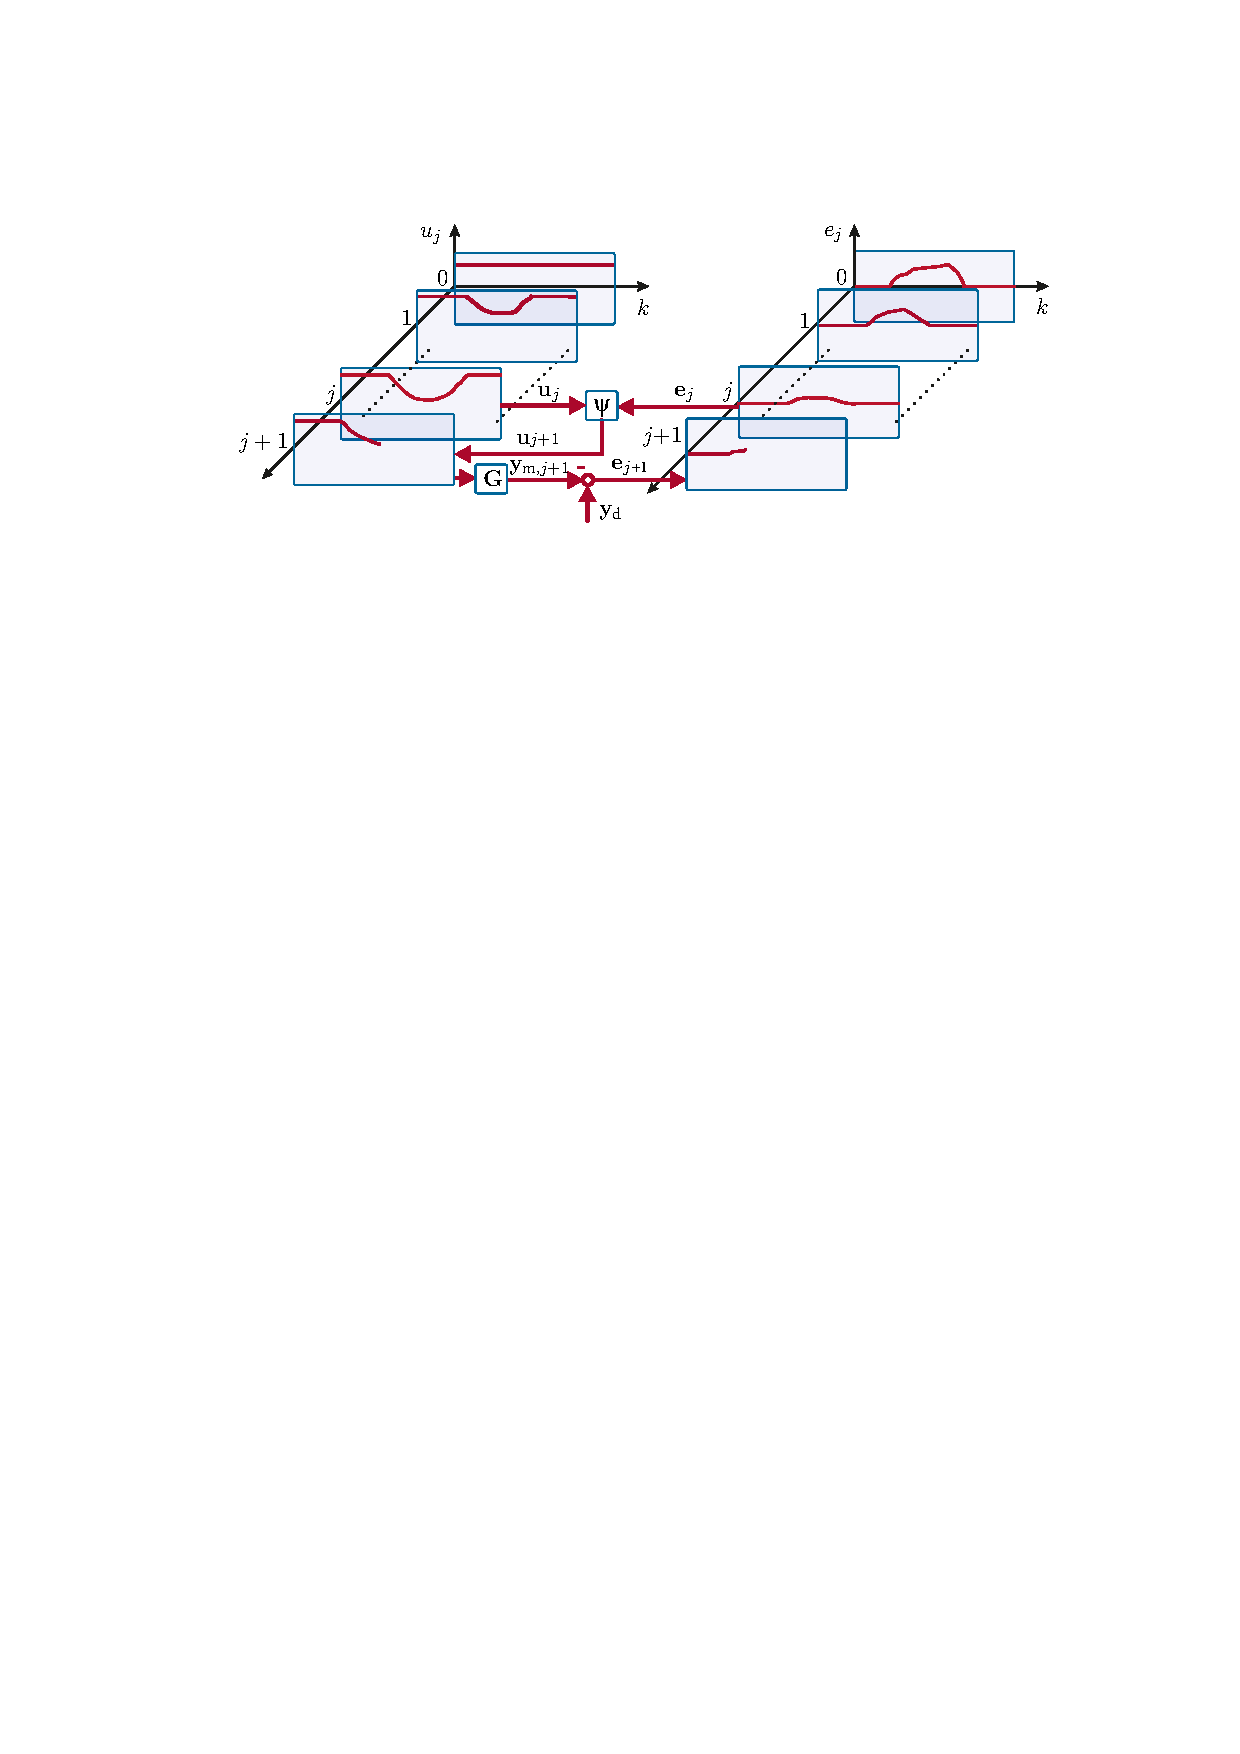
\includegraphics[width=1\textwidth]{./Bilder/Grundidee_ILC}
	\caption{Grundidee ILC \cite{UniWien}}
	\label{png:idee_ILC}
\end{figure}
In jeder Iteration wird die Steuerung $\uv_{j+1}$ durch die Funktion $\psi\bigl(\uv_j,\e_j(\uv_j)\bigr)$ berechnet. Die neue Steuerung ist somit nur von der vorherigen Iteration abhängig. Das daraus resultierende Stellsignal wird auf das System $\G$ angewendet, um den Ausgang $\y_{\mathrm{m},j+1}$ zu messen. Anhand des Sollsignals $\y_\mathrm{d}$ wird der neue Ausgangsfehler $\e_{j+1}$ ermittelt und zwischengespeichert. Gleichzeitig wird auch das an das System übergebene Stellsignal $\uv_{j+1}$ abgespeichert. Dieser Prozess kann beliebig oft wiederholt werden, wobei das Ziel darin besteht, die Steuerung $\uv$ so anzupassen, dass der Ausgangsfehler $\e$ gegen null konvergiert. \\
Die Berechnung des Stellsignals anhand einer Minimierungsaufgabe wird in den Vorlesungsunterlagen der Technischen Universität (TU) Wien \cite[9]{UniWien} hergeleitet und im Folgenden als gegeben angenommen. Zum Verständnis der Gleichung wird eine Verstärkungsmatrix $\Lm \in R^{N \times N}$ und eine Filtermatrix $\Q \in R^{N \times N}$ definiert, wobei $N$ die Anzahl der Abtastschritte während einer Iteration darstellt.\\
Das ILC-Gesetz hängt bei seiner Herleitung vom relativen Grad $r$ des Systems ab, welcher bei linearen Systemen auch als Polüberschuss bekannt ist. Für lineare zeitkontinuierliche Systeme kann der relative Grad mit der Gleichung
\begin{equation}
	\label{eq:r}
	r = n-m
\end{equation}
berechnet werden, wobei der höchste Exponent des Zählerpolynoms der Übertragungsfunktion durch $m$ und der höchste Exponent des Nennerpolynoms durch $n$ gegeben ist. Für zeitdiskrete Systeme gilt immer $r=1$. Der relative Grad eines diskreten Systems gibt den Zeitindex $r$ an, ab dem eine direkte Wirkung des Eingangs auf den Ausgang erfolgt. Er kann daher auch als Verzögerung interpretiert werden. \\
In praktischen Anwendungen kann es neben der Verzögerung durch den relativen Grad $r$ des Systems auch zu Verzögerungen aufgrund von Digital-Analog- oder Analog-Digital-Wandlungen kommen. Diese Verzögerung ist durch die Anzahl der Abtastschritte $w$ gegeben, welche für die Wandlung benötigt werden. Damit kann eine Gesamtverzögerung
\begin{equation}
	\label{eq:m}
	v = r + w
\end{equation}
eingeführt und im ILC-Gesetz berücksichtigt werden. \\

Mit der Definition der Vektoren:
\begin{align}
	\label{eq:u_vec}
	\uv_j &= \bigl[u_j[0] \quad u_j[1] \,  \ldots \, u_j[N-1] \bigr]^T \in R^{N \times 1} \\
	\yv_{\mathrm{d},j} &= \bigl[y_{\mathrm{d},j}[v] \quad y_{\mathrm{d},j}[v+1] \, \ldots \, y_{\mathrm{d},j}[v+N-1] \bigr]^T \in R^{N \times 1} \\
	\yv_{\mathrm{m},j} &= \bigl[y_{\mathrm{m},j}[v] \quad y_{\mathrm{m},j}[v+1] \, \ldots \, y_{\mathrm{m},j}[v+N-1] \bigr]^T \in R^{N \times 1} \\
	\ev_{j} &= \yv_{\mathrm{d},j} - \yv_{\mathrm{m},j} = \bigl[e_{j}[v] \quad e_{j}[v+1] \, \ldots \, e_{j}[v+N-1] \bigr]^T \in R^{N \times 1} \label{eq:evec_def}
\end{align}
ergibt sich das ILC-Gesetz in der Lifted-System Darstellung zu:
\begin{equation}
	\label{eq:ilc_lift}
	\uv_{j+1} = \Q\left(\uv_j + \Lm \e_j\right).
\end{equation}
Die Verstärkungsmatrix $\Lm$ hat die Aufgabe, den Einfluss des Ausgangsfehlers $\e_j$ in Relation zur vorherigen Steuerung $\uv_j$ zu bestimmen. Durch die Wahl der Matrixelemente kann also gesteuert werden, wie stark der Einfluss des Ausgangsfehlers auf die neue Steuerung ist. Die Filtermatrix $\Q$ dient hingegen dazu, Messrauschen und sich wiederholende Störungen zu unterdrücken. Dabei wirkt sie wie ein Tiefpassfilter, welcher nur niedrige Frequenzen passieren lässt und hohe Frequenzen herausfiltert. \\
Das ILC-Gesetz \autoref{eq:ilc_lift} kann auch in der diskreten Form angegeben werden:
\begin{equation}
	\label{eq:ilc_diskret}
	u_{j+1}[k] = q[k] \bigl(u_j[k] + l[k] \, e_j[k+v]\bigr).
\end{equation}
Dafür wird der Abtastindex $k = 0,1,\ldots,N-1$ definiert.
\section{Stabilität und Konvergenz}
In diesem Abschnitt werden die Stabilitäts- und Konvergenzkriterien aufgezeigt. Die Gleichungen sind den Vorlesungsunterlagen der TU Wien entnommen \cite{UniWien}. \\
Um die Stabilitäts- und Konvergenzkriterien zu überprüfen, wird die Impulsantwort $\g$ des Systems benötigt. Aus der Impulsantwort kann die Matrix  
\begin{equation}
	\label{eq:G}
	\G = \left( \begin{array}{cccc}
		\g[v] & 0 &  \cdots & 0 \\
		\g[v+1] & \g[v] &  \cdots & 0 \\
		\vdots & \vdots & \ddots & 0 \\
		\g[v+N-1] & \g[v+N-2] & \cdots & \g[v] \\
	\end{array}\right) \in R^{N \times N}
\end{equation}
gebildet werden. Es ist wichtig zu beachten, dass $\g[v] \neq 0$ gilt. Für die Berechnungen wird zusätzlich die Einheitsmatrix $\E \in R^{N \times N}$ herangezogen. \\
\\
Die Stabilität des ILC-Gesetzes \autoref{eq:ilc_lift} kann über \autoref{s:eingang_stabil} und \autoref{s:ausgang_stabil} nachgewiesen werden. Dafür wird als Hilfe der Spektralradius $\rho$ verwendet. Dieser ist definiert als der betragsmäßig größte Eigenwert einer quadratischen Matrix und kann wie folgt berechnet werden \cite{spektralradius}:
\begin{equation}
	\label{eq:spektralradius}
	\rho\left(\A\right) = \text{max} \, |\lambda_i\left(\A\right)|
\end{equation}
\begin{satz}[Stabilität der Eingangsfehleriteration]
	\label{s:eingang_stabil}
	Die Eingangsfehleriteration des ILC-Gesetzes, angewendet auf die Lifted-System Darstellung \ref{eq:ilc_lift} ist asymptotisch stabil, falls:
	\begin{equation}
		\label{eq:eingang_stabil}
		\rho\left(\Q\left(\E-\Lm\G\right)\right) < 1
	\end{equation}
\end{satz}
\begin{satz}[Stabilität der Ausgangsfehleriteration]
	\label{s:ausgang_stabil}
	Die Ausgangsfehleriteration des ILC-Gesetzes, angewendet auf die Lifted-System Darstellung \ref{eq:ilc_lift} ist asymptotisch stabil, falls:
	\begin{equation}
		\label{eq:ausgang_stabil}
		\rho\left(\G\Q\left(\E-\Lm\G\right)\G^{-1}\right) < 1
	\end{equation}
\end{satz}
Eine Gegenüberstellung der Eingangs- und der Ausgangsfehleriteration ergibt, dass die Matrizen aus \autoref{s:eingang_stabil} und \autoref{s:ausgang_stabil} dieselben Eigenwerte aufweisen. Dies bedeutet, dass die asymptotische Stabilität der Eingangsfehleriteration automatisch die asymptotische Stabilität der Ausgangsfehleriteration nachweist. Deshalb muss nur die Stabilität für eine Fehleriteration nachgewiesen werden. \\
\\
Die Konvergenz ist über \autoref{s:konv_u} und \autoref{s:konv_e} nachweisbar. Dafür wird der maximale Singulärwert $\bar{\sigma}$ einer Matrix $\A$ benötigt. Der maximale Singulärwert dieser Matrix entspricht dabei ihrer Spektralnorm und kann daher mit
\begin{equation}
	\label{eq:singulärwert}
	\bar{\sigma} = \sqrt{\text{max} \, |\lambda_i\left(\A^T\A\right)|}
\end{equation}
berechnet werden \cite{spektralnorm}. \\
Zur Berechnung des maximalen Singulärwerts einer Matrix in Matlab kann die Funktion \lstinline{svd(A)} verwendet werden. Die Funktion führt eine Singulärwertzerlegung durch und gibt alle Singulärwerte zurück. Um nur den gewünschten maximalen Singulärwert zu erhalten, kann die Funktion \textit{max} benutzt werden \cite{MATLAB}. Dadurch wird nur der größte Singulärwert zurückgegeben, siehe \autoref{lst:maximalersingulaerwert}: 
\lstinputlisting[language= Matlab, firstline=3, lastline=3, numbers=none, caption={Berechnung maximaler Singulärwert}, label=lst:maximalersingulaerwert]{Latex.m}
\begin{satz}[Monotone Konvergenz der Eingangsfehleriteration]
	\label{s:konv_u}
	Die Eingangs\-fehleriteration der Lifted-System Darstellung \ref{eq:ilc_lift} ist monoton konvergent gegen $\uv_{\infty}$, wenn gilt:
	\begin{equation*}
		\label{eq:konv_u_1}
		\|\uv_{j+1} - \uv_{\infty}\|_2 \leq \alpha \|\uv_{j} - \uv_{\infty}\|_2
	\end{equation*}
	für $ 0 \leq \alpha < 1$ 
	\begin{equation}
		\label{eq:konv_u}
		\bar{\sigma}\left(\Q\left(\E-\Lm\G\right)\right) < 1
	\end{equation}
\end{satz}
\begin{satz}[Monotone Konvergenz der Ausgangsfehleriteration]
	\label{s:konv_e}
	Die Ausgangs\-fehler\-itera\-tion der Lifted-System Darstellung \ref{eq:ilc_lift} ist konvergent gegen $\e_{\infty}$, wenn gilt:
	\begin{equation*}
		\label{eq:konv_e_1}
		\|\e_{j+1} - \e_{\infty}\|_2 \leq \beta \|\e_{j} - \e_{\infty}\|_2
	\end{equation*}
	für $ 0 \leq \beta < 1$ 
	\begin{equation}
		\label{eq:konv_e}
		\bar{\sigma}\left(\G\Q\left(\E-\Lm\G\right)\G^{-1}\right) < 1
	\end{equation}
\end{satz}
Für den Beweis der monotonen Konvergenz in \autoref{s:konv_u} und \autoref{s:konv_e}, werden die gleichen Matrizen wie in \autoref{s:eingang_stabil} und \autoref{s:ausgang_stabil} verwendet. Daraus folgt, dass die Matrizen die gleichen Singulärwerte besitzen und es ausreicht, monotone Konvergenz für eine Fehleriteration nachzuweisen. \\
Wenn die Stabilitäts- und Konvergenzkriterien erfüllt sind, kann der asymptotische Ausgangsfehler laut de Castro und T\^{o}rres \cite{ilc_anwendung} mit
\begin{equation}
	\label{eq:e_inf}
	\e_{\infty} = \left(\E-\G\left(\E-\Q\left(\E-\Lm\G\right)\right)^{-1}\Q\Lm\right)\left(\y_\mathrm{d} - \y_{\mathrm{m},0}\right)
\end{equation}
berechnet werden. Dafür wird der Anfangszustand $\y_{\mathrm{m},0}$ des Istsignals benötigt. Der Ausgangsfehler kann nur zu null werden, wenn keine Filterung durchgeführt wird, das heißt
\begin{equation}
	\label{eq:Q_E}
	\Q = \E \qquad \rightarrow \qquad \e_{\infty} = 0.
\end{equation}
Die Verwendung eines Filters im ILC-Gesetz führt dazu, dass der Regelfehler nicht auf null konvergieren kann. Dies liegt daran, dass der Filter den Ausgang des Systems glättet und somit die hochfrequenten Anteile des Regelfehlers reduziert. Dadurch wird auch die Fähigkeit der Regelung beeinträchtigt auf hochfrequente Änderungen zu reagieren. In praktischen Anwendungen ist es allerdings häufig notwendig, einen Filter je nach Anwendung zu verwenden, um Rauschen und Störungen zu unterdrücken. In diesem Fall ist es wichtig, eine geeignete Filtermatrix zu wählen, welche die unerwünschten Frequenzen herausfiltert, während gleichzeitig eine ausreichende Regelgenauigkeit erreicht werden kann.

\section{ILC-Gesetze}
In diesem Abschnitt geht es um die verschiedenen Arten von ILC-Gesetzen, die in der Praxis eingesetzt werden können. Es werden drei Arten von ILC-Gesetzen beschrieben. \\
Die P-Type und PD-Type Iterative Learning Control verwenden bekannte Konzepte der PID-Ausgangsregelung. Dabei wird der Ausgangsfehler $\e_j$, je nach Typ der Regelung,  proportional und/oder differentiell zurückgeführt. Es wird jedoch in der Regel kein Integralanteil verwendet, da das ILC-Gesetz, durch die Aufsummierung des Stellsignals, bereits ein integrierendes Verhalten aufweist und somit die Vorteile des I-Anteils besitzt. Eine stationäre Genauigkeit ist somit bereits gegeben. \\
Das dritte Konzept ist das sogenannte inversionsbasierte Konzept, welches auf Basis des invertierenden Modells der Regelstrecke aufgebaut ist.\\
Außerdem wird der Entwurf einer akausalen Filterung erläutert.
\subsection{P-Type}
Wie auch bei einem klassischen Feedbackregler, ist das einfachste ILC Gesetz ein P-Type. Dabei wird die Verstärkungsmatrix $\Lm$ zur einer diagonalen Verstärkungsmatrix mit dem Verstärkungsfaktor $k_\mathrm{p} > 0$ gewählt.
\begin{equation}
	\label{eq:L_p}
	\Lm = k_\mathrm{p} \E
\end{equation}
Daraus ergibt sich aus \autoref{eq:ilc_lift} das P-Type ILC-Gesetz in der Lifted-System Schreibweise zu

\begin{equation}
	\label{eq:ilc_p}
	\uv_{j+1} = \Q \left( \uv_j + k_\mathrm{p}  \E \, \e_j \right).
\end{equation}
und analog dazu die diskrete Darstellung
\begin{equation}
	\label{eq:ilc_p_k}
	u_{j+1}[k] = q[k] \bigl(u_j[k] + k_\mathrm{p} \, e_j[k+v] \bigr).
\end{equation}

\subsection{PD-Type}
Die PD-Type Iterative Learning Control verwendet sowohl den Ausgangsfehler als auch eine numerische Approximation der Zeitableitung des Ausgangsfehlers. Es ist daher eine Kombination aus Proportional- und Differentialglied. Um den Differenzialanteil einzustellen, wird die Verstärkungsmatrix $\Lm$ um einen zusätzlichen Einstellparameter $k_\mathrm{d} > 0$ und einer Ableitungsfiltermatrix $\Dm$ erweitert. Daraus ergibt sich
\begin{equation}
	\label{eq:L_pd}
	\Lm = k_\mathrm{p} \E + k_\mathrm{d} \Dm.
\end{equation}
Je nach gewähltem zeitdiskreten Ansatz für die Gestaltung der Matrix $\Dm$ kann diese unterschiedlich strukturiert sein. Im Folgenden ist beispielhaft ein möglicher Aufbau der Ableitungsfiltermatrix dargestellt:
\begin{equation}
	\label{eq:D}
	\Dm = \frac{1}{T_\mathrm{s}}\left( \begin{array}{ccccc}
		$-$1 & 1 & 0 & \cdots & 0 \\
		$-$\frac{1}{2} & 0 & \frac{1}{2} & \cdots & 0 \\
		\vdots & \ddots & \ddots & \ddots & 0 \\
		0 & 0 & $-$\frac{1}{2} & 0 & \frac{1}{2} \\
		0 & 0 & 0 & $-$1 & 1\\
	\end{array}\right) \in R^{N \times N}.
\end{equation}
Die Schrittweite ist dabei durch die Variable $T_\mathrm{s}$ gegeben.\\
Aus \autoref{eq:ilc_lift} ergibt sich das PD-Type ILC-Gesetz in der Lifted-System Darstellung zu
\begin{equation}
	\label{eq:ilc_pd}
	\uv_{j+1} = \Q \left( \uv_j + \left(k_\mathrm{p}  \E  +  k_\mathrm{d} \Dm \right) \e_j \right)
\end{equation}
und analog dazu die diskrete Schreibweise
\begin{equation}
	\label{eq:ilc_pd_k}
	u_{j+1}[k] = q[k] \left(u_j[k] + k_\mathrm{p} \, e_j[k+v] + \frac{k_\mathrm{d}}{2T_\mathrm{s}}\left(e_j[k+v+1] - e_j[k+v-1]  \right) \right).
\end{equation}

\subsection{Inversionsbasiertes ILC}
Inversionsbasiertes Iterative Learning Control ist eine Erweiterung des klassischen ILC-Konzepts, bei dem das invertierte Modell der Regelstrecke verwendet wird. Dafür muss die Impulsantwort $\g$ der Regelstrecke und damit auch die Matrix $\G$ bekannt sein. Für das ILC-Gesetz bedeutet dies, dass die Verstärkungsmatrix $\Lm$ zur inversen Matrix von $\G$ gewählt wird: 
\begin{equation}
	\label{eq:L_Ginv}
	\Lm = \G^{-1}.
\end{equation}
Dadurch ergibt sich aus \autoref{eq:ilc_lift} das inversionsbasierte ILC-Gesetz in der Lifted System Schreibweise zu
\begin{equation}
	\label{eq:ilc_G}
	\uv_{j+1} = \Q \left( \uv_j + \G^{-1} \e_j \right).
\end{equation}
Mit diesem Verfahren ist es möglich, den Ausgangsfehler $\e_j$ in einer Iteration auf den Grenzwert $\e_{\infty}$ zu bringen. Wenn die Filtermatrix zu $\Q = \E$ gewählt wird, gilt zudem $\e_{\infty} = 0$. Allerdings ist dies in der Praxis oft schwer realisierbar, da in realen Anwendungen $\G$ nie exakt bekannt und der Einsatz eines Filters essentiell ist.

\subsection{Akausale Filterung}
Der Einsatz einer Filterung hat den Zweck, das Lernen von nicht wiederkehrenden Störungen und Messrauschen zu unterbinden. Dies erweist sich insbesondere als relevant, wenn der ILC-Ansatz auf realer Hardware eingesetzt wird.\\
Wie bereits erwähnt, können für die Filterung auch akausale Filter verwendet werden.  Ein einfacher Ansatz für einen akausalen Tiefpassfilter besteht in der Anwendung eines Gauß-Filters \cite{UniWien}. Dafür wird die diskrete Gauß-Verteilung 
\begin{equation}
	\label{eq:disc_gaus_ver}
	\q_\mathrm{G}[k] = \frac{T_\mathrm{s}}{\sigma_\mathrm{q}\sqrt{2\pi}} \, \exp\left(-\frac{\left(kT_\mathrm{s}\right)^2}{2\sigma_\mathrm{q}^2}\right)
\end{equation}
mit der Standartabweichung 
\begin{equation}
	\label{eq:standabweichung}
	\sigma_\mathrm{q} = \frac{\sqrt{\ln(2)}}{2\pi f_\mathrm{c}}
\end{equation}
verwendet. Hierbei steht der Parameter $f_\mathrm{c}$ für die Grenzfrequenz und bestimmt die Bandbreite bis zur -3dB-Absenkung. \\
Um eine Fensterung mit einer Länge von $2N\mathrm{q}+1$ zu erhalten, ergibt sich der Vektor für den Gaußfilter zu
\begin{equation}
	\label{eq:disc_gaus}
	\q[k] = \frac{\q_\mathrm{G}[k]}{\sum_{m = -N_\mathrm{q}}^{N_\mathrm{q}}\q_\mathrm{G}[m]} \in R^N.
\end{equation}
Mithilfe des Vektors $\vec{q}$ kann die Filtermatrix $\Q$ konstruiert werden. Hierfür werden die Parameter $N$ und $N_\mathrm{q}$ verwendet. Im Folgenden ist ein Beispiel für die Erstellung einer Filtermatrix mit $N=5$ und $N_\mathrm{q}=2$ gegeben:
\begin{equation}
	\label{eq:filtermatrix}
	\Q = \left( \begin{array}{cccccc}
		\q[0] & \q[-1] & \q[-2] & 0 	 & 0\\
		\q[1] & \q[0]  & \q[-1] & \q[-2] & 0\\
		\q[2] & \q[1]  & \q[0]  & \q[-1] & \q[-2] \\
		0	 & \q[2]  & \q[1]  & \q[0]  & \q[-1] \\
		0 	 & 0 	 & \q[2]  & \q[1]  & \q[0] \\
	\end{array}\right) \in R^{5 \times 5}.
\end{equation}
\section{Matlab-Simulink}
Dieses Kapitel stellt die Matlap Skripte zur Untersuchung der Stabilität- und Konvergenzkriterien sowie das Simulink Modell mit dem ILC-Ansatz vor. Für die vorliegende Abschlussarbeit wurde die Matlab Version 2021a verwendet. \\
Für alle weiteren Untersuchungen wird das in \autoref{png:Sollsignal} dargestellte Sollsignal $\yv_\mathrm{d}$ eingesetzt. 
\begin{figure}[ht]
	\centering
	\includegraphics[width=1\textwidth]{./Bilder/Sollsignal}
	\caption{Sollsignal}
	\label{png:Sollsignal}
\end{figure}
Das Sollsignal besteht aus einer Sinusschwingung, einer sprungförmigen Ansteigung und einer rampenförmigen Ansteuerung. Dadurch kann das Systemverhalten für unterschiedliche Signalarten überprüft werden. Die Kanten sind durch die Faltung mit einem Gausfilter etwas abgeflacht. In der Praxis wird dies durch die Bahnplanung vorgenommen. Die Periodendauer des Sollsignals beträgt 42 Sekunden.

\subsection{Untersuchung Stabilität und Konvergenz}
Zur Untersuchung der Stabilitäts- und Konvergenzkriterien wurde ein Skript erstellt, welches aus einer gegebenen Übertragungsfunktion die Impulsantwort berechnet und für die unterschiedlichen ILC-Gesetze die zulässigen Parameter $k_\mathrm{p}$ und gegebenenfalls $k_\mathrm{d}$ bestimmt. Anschließend werden die Ergebnisse in einem Schaubild aufgezeigt. In \autoref{lst:stab_konv} ist ein Ausschnitt aus dem Matlab Skript zur Parameterbestimmung abgebildet. 
\lstinputlisting[language= Matlab, firstline=6, lastline=30,caption={Untersuchung Stabilität und Konvergenz}, label=lst:stab_konv]{Latex.m}
Zu Beginn wird versucht, die Stabilitäts- und Konvergenzkriterien eines P-Type ILC zu erfüllen. Dafür sind die Einheitsmatrix $\E$ und die Matrix $\G$ bereits definiert und berechnet. Die Matrix $\G$ berechnet sich  aus einer gegebenen Übertragungsfunktion. Durch den Vektor \lstinline{kp_test} wird eine Wertespanne festgelegt, für die der Parameter $k_\mathrm{p}$ überprüft werden soll. In einer Vorschleife wird die Verstärkungsmatrix $\Lm$ für jeden gewünschten $k_\mathrm{p}$-Wert berechnet. In den Zeilen acht und neun werden die Stabilitäts- und Konvergenzkriterien gemäß den Gleichungen \ref{eq:eingang_stabil} und \ref{eq:konv_u} bestimmt. Die berechneten Werte werden in Vektoren gespeichert, um sie später in einem Schaubild darzustellen. In Zeile zehn werden die Stabilitäts- und Konvergenzkriterien gemäß \autoref{s:eingang_stabil} und \autoref{s:konv_u} überprüft. Wenn beide Kriterien erfüllt sind, wird der $k_\mathrm{p}$-Wert in einer Liste abgespeichert. Außerdem wird die asymptotische Regelabweichung mit Hilfe von \autoref{eq:e_inf} bestimmt und der maximale Wert und der Effektivwert des Vektors gebildet. Wenn kein passender $k_\mathrm{p}$-Wert gefunden werden kann, wird im nächsten Schritt ein sehr ähnlicher Ablauf für ein PD-Type ILC durchgeführt.

\subsection{Simulink-Modell ILC-Ansatz}
\label{subsec_simulink_modell}
In diesem Abschnitt wird das Matlab-Simulink Modell mit dem ILC-Ansatz betrachtet, welches in \autoref{png:mat_ilc_ansatz} dargestellt ist. Das Modell besteht aus zwei Subsystemen. Im grünen Subsystem wird das Sollsignal gemäß \autoref{png:Sollsignal} mit einer Abtastrate $T_\mathrm{s}$ am Ausgang ausgegeben. Das orangene Subsystem ist ein sogenanntes Resettable Subsystem, welches über den oberen Eingang ein- oder ausgeschaltet werden kann. Dieses Subsystem enthält den ILC-Ansatz.
\begin{figure}[H]
	\centering
	\includegraphics[width=1\textwidth]{./Bilder/Matlab_ILC_Ansatz}
	\caption{Matlab Modell ILC-Ansatz}
	\label{png:mat_ilc_ansatz}
\end{figure}
Als Eingänge erhält der Block das Sollsignal $y_\mathrm{d}$ und das gemessene Signal $y_\mathrm{m}$. Als Ausgänge werden das Stellsignal $u_k$, welches direkt auf die Regelstrecke wirkt, und der Regelfehler $\e$ bereitgestellt. Der Regelfehler $\e$ ist ein Vektor, der die aktuelle Regelabweichung $e_k$, die maximale Regelabweichung $e\Max$ und den Effektivwert \textit{Root Mean Square} $e_\mathrm{rms}$ der letzten Iteration enthält.\\
Der ILC-Ansatz arbeitet im diskreten Zeitbereich, deshalb wird die Regelstrecke als diskrete Übertragungsfunktion angegeben. Dafür muss die kontinuierliche Übertragungsfunktion $G_\mathrm{s}(s)$ in eine diskrete Übertragungsfunktion $G_\mathrm{s}(z)$ transformiert werden.
\subsubsection{Maske}
Die Maske ist eine grafische Benutzeroberfläche, die es ermöglicht, die Einstellungen und Parameter eines Simulink-Blocks zu konfigurieren. In diesem Fall wird die Maske verwendet, um die benötigten Parameter an den ILC-Block zu übergeben (siehe \autoref{png:mat_ilc_maske}).
\begin{figure}[ht]
	\centering
	\includegraphics[width=0.5\textwidth]{./Bilder/ILC_Maske}
	\caption{ILC Subsystem Maske}
	\label{png:mat_ilc_maske}
\end{figure}
Der Parameter \textit{Modus} ermöglicht die Auswahl zwischen verschiedenen ILC-Typen, während der Parameter \textit{Filterung} entscheidet, ob eine Filterung des Signals vorgenommen werden soll oder nicht. Im vorherigen Kapitel wurde der D-Typ ILC-Ansatz nicht detailliert behandelt, jedoch nun aus Testzwecken aufgenommen. Für den inversionsbasierten ILC-Ansatz wird die Impulsantwort $\g$ der Übertragungsfunktion, welche zuvor berechnet werden muss, im Hintergrund in den ILC-Block geladen.
\subsubsection{ILC-Algorithmus}
Innerhalb des orangenen Subsystems befindet sich eine Matlab-Funktion (siehe \autoref{lst:ilc_algo}), welche den ILC-Algorithmus enthält. 
\lstinputlisting[language= Matlab, firstline=32, lastline=94,caption={ILC-Algorithmus}, label=lst:ilc_algo]{Latex.m}
Die Funktion erhält als Eingangsparameter die Eingänge des Subsystems sowie die in der Maske definierten Parameter. Die Ausgabeparameter der Funktion entsprechen den Ausgängen des Subsystems. Zunächst werden die internen Variablen definiert und über die \lstinline{if isempty(...)} Abfrage initialisiert. Die Filtermatrix $\Q$ und die Ableitungsmatrix $\Dm$ werden in einer externen Funktion berechnet und bei der Initialisierung geladen. \\
Der eigentliche ILC-Algorithmus beginnt ab Zeile 21. Zunächst wird das neue Stellsignal \lstinline{u_k} aus dem Vektor \lstinline{Useq} mithilfe des Abtastindex \lstinline{k} extrahiert. Danach wird der Regelfehler \lstinline{e_k} mit \autoref{eq:e_yd_ym} berechnet und in einem Vektor \lstinline{e} abgespeichert. Zur Bestimmung des maximalen Regelfehlers \lstinline{e_max} und des Effektivwertes der Regelabweichung \lstinline{e_rms} werden zusätzliche lokale Variablen benötigt, damit die Berechnung am Ende jeder Iteration stattfinden kann.\\
In Zeile 31 wird der Abtastindex \lstinline{k} um eins erhöht. Durch die Verschiebung des Regelfehlers \lstinline{e} um die Verzögerung \lstinline{v}, verschiebt sich ein Teil des Stellsignals in die vorherige Iteration. Ab Zeile 32 wird das vorgezogene Stellsignal für das Ende der aktuellen Iteration berechnet. Dafür wird abhängig vom eingestellten Modus die Gleichung \ref{eq:ilc_p}, \ref{eq:ilc_pd} oder \ref{eq:ilc_G} verwendet.\\
Zuletzt erfolgt die Überprüfung, ob der Abtastindex \lstinline{k} größer als die maximale Anzahl der Schritte \lstinline{Nseq} ist. Trifft dies zu, wird der Abtastindex auf eins zurückgesetzt und das neue Stellsignal wird berechnet. Dafür wird der Vektor \lstinline{e} um die Verzögerung \lstinline{v}, laut \autoref{eq:evec_def} verschoben. Anschließend wird, abhängig davon welcher Modus in der Maske ausgewählt wird, das neue Stellsignal \lstinline{Useq} berechnet. Je nach Einstellung des \lstinline{filt} Parameters in der Maske, wird die Filtermatrix $\Q$ in Zeile 60 auf das neu berechnete Stellsignal angewendet. Dadurch wird das Signal unabhängig vom eingestellten Modus gefiltert.

\subsection{Simulink-Modell ILC-Ansatz + PID-Regler}
\label{subsec_modell_ilc_pid}
Das in \autoref{png:mat_ilc_ansatz} gezeigte Modell wird um einen Feedback-Anteil erweitert. Dafür wird ein klassischer PID-Regler eingesetzt. Hierbei gibt es zwei verschiedene Strukturen, die angewendet werden können. Bei der parallelen Struktur (\autoref{png:mat_ilc_pid_parallel}), welche auch als Zwei-Freiheitsgrade-Regelung bezeichnet wird, wird der ILC-Anteil zum Ausgang des Reglers addiert. Anders ist es bei der seriellen Struktur (\autoref{png:mat_ilc_pid_seriell}); hier wird der ILC-Anteil zum Eingang des Reglers addiert. Die parallele Struktur wird als Zwei-Freiheitsgrade-Regelung bezeichnet.
\begin{figure}[H]
	\centering
	\includegraphics[width=1\textwidth]{./Bilder/Matlab_ILC_Ansatz_PID_parallel.pdf}
	\caption{Matlab Modell ILC-Ansatz mit PID-Regler in paralleler Struktur}
	\label{png:mat_ilc_pid_parallel}
\end{figure}
\begin{figure}[H]
	\centering
	\includegraphics[width=1\textwidth]{./Bilder/Matlab_ILC_Ansatz_PID_seriell.pdf}
	\caption{Matlab Modell ILC-Ansatz mit PID-Regler in serieller Struktur}
	\label{png:mat_ilc_pid_seriell}
\end{figure}

\section{Ergebnisse}
In diesem Abschnitt werden die Ergebnisse aus der Untersuchung der Stabilitäts- und Konvergenzkriterien präsentiert. Dabei wird außerdem der ILC-Algorithmus an verschiedenen Regelstrecken mit unterschiedlichen ILC-Gesetzen getestet. Die Regelfehlerverläufe und die Konvergenzgeschwindigkeiten der Regelung sollen hierbei unter anderem untersucht und verglichen werden. Außerdem wird die Kombination aus ILC-Ansatz und PID-Regelung simuliert und ebenfalls untersucht. Bei den Simulationen wird der ILC-Ansatz ohne Filterung ($\Q = \E$) eingesetzt.
\subsection{PT1-System}
Als erstes wird der ILC-Ansatz an einem System mit PT1-Verhalten untersucht. Die Übertragungsfunktion im kontinuierlichen Zeitbereich der Regelstrecke $G_\mathrm{s}(s)$ ist gegeben durch 
\begin{equation}
	\label{eq:ilc_Gs_pt1}
	G_\mathrm{s}(s) = \frac{0.1}{0.4s+1.1}.
\end{equation}
Wie in \autoref{subsec_simulink_modell} erläutert, wird bei der Simulation die Regelstrecke im diskreten Zeitbereich benötigt. Dafür muss die kontinuierliche Übertragungsfunktion $G_\mathrm{s}(s)$ mithilfe der Z-Transformation in eine diskrete Übertragungsfunktion $G_\mathrm{s}(z)$ transformiert werden. Dies kann zum Beispiel durch eine Rechteck-Vorwärts-Transformation, auch Euler-Transformation genannt, der kontinuierlichen Übertragungsfunktion mit $s = \frac{1}{T_\mathrm{s}}\left(z-1\right)$ erfolgen \cite{Skript_Baur}. In Matlab kann die kontinuierliche Übertragungsfunktion mit dem Befehl \lstinline{c2d(Gs, Ts)} in den diskreten Zeitbereich transformiert werden. Für die Untersuchungen und Simulationen wird eine Abtastzeit von $T_\mathrm{s} = \unit[0.1]{s}$ gewählt. Dadurch ergibt sich die diskrete Übertragungsfunktion (bestimmt mit Matlab) zu
\begin{equation}
	\label{eq:ilc_Gz_pt1}
	G_\mathrm{s}(z) = \frac{0.02186}{z - 0.7596}.
\end{equation}
\subsubsection{P-Type ILC}
\label{subsub:P_type}
Zunächst wird der P-Typ ILC-Ansatz am System angewendet, wobei der Parameter $k_\mathrm{p}$ durch \autoref{lst:stab_konv} eingegrenzt wird. Die Ergebnisse der Untersuchung sind in \autoref{png:erg_pt1_stab_konv} dargestellt. Im oberen und unteren Diagramm sind die Auswirkungen des Parameters $k_\mathrm{p}$ auf die Stabilität, Konvergenz und der asymptotischen Regelabweichung ($e_{\textrm{max},\infty}$ und $e_{\mathrm{rms},\infty}$) des Systems zu sehen.
\begin{figure}[H]
	\centering
	\includegraphics[width=0.9\textwidth]{./Bilder/Untersuchung_PT1_Glied}
	\caption{Stabilitäts- und Konvergenzuntersuchung PT1-System}
	\label{png:erg_pt1_stab_konv}
\end{figure}
Das obere Diagramm zeigt die Stabilitäts- und Konvergenzergebnisse für verschiedene $k_\mathrm{p}$-Werte. Um die Stabilitäts- und Konvergenzkriterien zu erfüllen, muss der berechnete Wert kleiner als eins sein (vgl. \autoref{s:eingang_stabil} und \autoref{s:konv_u}). Die Ergebnisse zeigen, dass der ILC-Ansatz für $k_\mathrm{p}$-Werte unter 22 stabil ist und eine monotone Konvergenz aufweist. Für Werte ab 22 ist zwar das Stabilitätskriterium weiterhin erfüllt, allerdings ist das Konvergenzkriterium nicht mehr erfüllt.\\
Im unteren Schaubild ist die maximale Regelabweichung und der Effektivwert der Regelabweichung in Abhängigkeit von $k_\mathrm{p}$ dargestellt. Je höher der $k_\mathrm{p}$-Wert, desto kleiner ist die Regelabweichung. Die Formel zur Berechnung der asymptotischen Regelabweichung ist nur anwendbar, solange die Stabilitäts- und Konvergenzkriterien erfüllt sind. Aus diesem Grund wurde ab einem $k_\mathrm{p}$-Wert von 22 keine Berechnung durchgeführt.\\
Die Ergebnisse zeigen, dass der P-Typ ILC-Ansatz mit einem $k_\mathrm{p}$-Wert im Bereich von $0 < k_\mathrm{p} < 22$ für die Strecke \ref{eq:ilc_Gs_pt1} beziehungsweise \ref{eq:ilc_Gz_pt1} eingesetzt werden kann, um eine stabile Regelung mit einer Konvergenz der Regelabweichung auf Werte im Bereich von $10^{-16}$ zu erreichen.\\
Diese theoretischen Untersuchungen werden im nächsten Schritt, anhand einer Simulation in Matlab-Simulink, untersucht. Dafür wird das Modell aus \autoref{png:mat_ilc_ansatz} mit der definierten diskreten Übertragungsfunktion \ref{eq:ilc_Gz_pt1} verwendet. Als P-Anteil wird ein $k_\mathrm{p}$-Wert von 4 eingestellt, welcher heuristisch bestimmt wurde. In \autoref{png:erg_p_pt1_sim} sind die Ergebnisse der Simulation zu sehen.
\begin{figure}[H]
	\centering
	\includegraphics[width=0.96\textwidth]{./Bilder/Messung_P_PT1_kp_4}
	%P_Typ_PT1_kp_4.mat
	\caption{Simulationsergebnis P-Typ ILC anhand PT1-System}
	\label{png:erg_p_pt1_sim}
\end{figure}
Im oberen Schaubild ist das Sollsignal $y_\mathrm{d}$ in rot und die gemessenen Signale $y_\mathrm{m}$, nach einer bestimmten Anzahl an Iterationen, dargestellt. Die Regelabweichung zwischen diesen Signalen, welche zu jedem Zeitschritt $k$ aufgezeigt wird, ist im mittleren Schaubild zu sehen. Das ILC-Gesetz hängt nur von der vorherigen Iteration ab, wodurch das Istsignal nach einer Iteration gleich null ist und die Regelabweichung dem Sollsignal entspricht. Mit zunehmender Anzahl von Iterationen nähert sich das gemessene Signal dem Sollsignal an und die Regelabweichung wird kleiner. Nach 20 Iterationen ist im oberen Schaubild fast kein Unterschied zwischen Sollsignal und gemessenem Signal erkennbar. Lediglich bei der impulsartigen Ansteigung ist ein kleiner Knick bei der Regelabweichung zu erkennen.\\
Im unteren Schaubild wird die Regelabweichung ($e\Max$ und $e_{\mathrm{rms}}$) in Abhängigkeit der Iterationen aufgezeigt. Die y-Achse ist dabei logarithmisch dargestellt. Mit zunehmender Anzahl von Iterationen wird die Regelabweichung kleiner. Nach 500 Iterationen erreicht der $e\Max$-Wert $2.5 \cdot 10^{-15}$ und der $e_{\mathrm{rms}}$-Wert $4.4 \cdot 10^{-16}$.\\
Die Wahl des Parameters $k_\mathrm{p}$ beeinflusst die Konvergenzgeschwindigkeit der Regelabweichung. Größere $k_\mathrm{p}$-Werte führen zu einer schnelleren Konvergenz, während kleinere Werte zu einer langsameren Konvergenz führen. Wenn der $k_\mathrm{p}$-Wert kurz unterhalb des erlaubten Bereichs liegt, kommt es zum Überschwingen des Istsignals im Vergleich zum Sollsignal, was ein vergleichbares Verhalten wie bei einer Sprungantwort eines PID-Reglers darstellt.\\
Für $k_\mathrm{p}$-Werte ab 22 konvergiert das Istsignal nicht und die Regelabweichung steigt ins Unendliche. Die Simulationsergebnisse stimmen mit den theoretischen Untersuchungen überein. 

\subsubsection{Inversionsbasiertes ILC}
Im Folgenden wird der inversionsbasierte ILC-Ansatz untersucht. Dafür wird der Modus vier in der Maske des ILC-Subsystems eingestellt. Die Ergebnisse der Simulation sind in \autoref{png:erg_ginv_pt1_sim} zu sehen. Das Schaubild hat den gleichen Aufbau wie die \autoref{png:erg_p_pt1_sim}.
\begin{figure}[H]
	\centering
	\includegraphics[width=0.96\textwidth]{./Bilder/Messung_P_PT1_G_inv}
	%G_inv_PT1.mat
	\caption{Simulationsergebnis Inversionsbasiertes ILC anhand PT1-System}
	\label{png:erg_ginv_pt1_sim}
\end{figure}
In den oberen beiden Schaubildern ist zu erkennen, dass bereits nach zwei Iterationen (einer Wiederholung) das Istsignal dem Sollsignal entspricht. Die Regelabweichung ist dabei auf ihren minimalen Wert konvergiert. 

\subsubsection{ILC-Ansatz + PI-Regler}
\label{subsubsec_ILC_PID}
In diesem Abschnitt erfolgt eine Untersuchung einer Kombination aus ILC-Ansatz und PI-Regler. Hierbei werden die Simulink-Modelle aus \autoref{subsec_modell_ilc_pid} in Verbindung mit der gegebenen diskreten Übertragungsfunktion \autoref{eq:ilc_Gz_pt1} verwendet. Die Einstellung der Regelparameter des PI-Reglers (ideal Struktur mit Anti-Wind-Up) erfolgt mittels der in Matlab verfügbaren PID Tuner App und wird durch verschiedene Simulationen in Kombination mit dem ILC-Ansatz angepasst. Es werden Werte von $6.1$ für den P-Anteil und $\unit[2.9]{s^{-1}}$ für den I-Anteil ermittelt. Der ILC-Ansatz wird für beide Untersuchungen als P-Type eingesetzt. Die $k_\mathrm{p}$-Parameter des ILC-Ansatzes wurden experimentell ermittelt.\\
Im ersten Schritt erfolgt eine Untersuchung der parallelen Struktur. Dafür wird ein Wert von $15$ für den $k_\mathrm{p}$-Parameter des ILC-Ansatzes eingestellt. Die Ergebnisse der Simulation sind in \autoref{png:erg_pt1_ilc_pid_parallel} dargestellt.
\begin{figure}[H]
	\centering
	\includegraphics[width=1\textwidth]{./Bilder/Messung_PT1_ILC_PID_parallel}
	%P_Typ_PT1_ILC_kp_15_PID_P_6_1_I_2_9_para.mat
	\caption{Simulationsergebnis ILC-Ansatz + PI-Regler in paralleler Struktur anhand PT1-System}
	\label{png:erg_pt1_ilc_pid_parallel}
\end{figure}
Die blauen Linien in den oberen beiden Diagrammen zeigen das Ergebnis der Regelung allein durch den PI-Regler (ILC-Ansatz benötigt eine Iteration bis er wirksam wird). Durch den ILC-Ansatz nähert sich das Istsignal, nach mehreren Iterationen, schrittweise dem Sollsignal an. Der Effektivwert und die maximale Regelabweichung betragen nach 500 Iterationen $7.2\cdot 10^{-4}$ und $1.0\cdot10^{-3}$. Die Regelgüte des PI-Reglers konnte somit signifikant verbessert werden.\\
Mittels Simulationen mit verschiedenen Reglerparametern wird festgestellt, dass der Integral-Anteil des Reglers der Konvergenzgeschwindigkeit der ILC-Methode entgegenwirkt. Bei Nullsetzung des Integral-Anteils des Reglers kann die Konvergenzgeschwindigkeit erhöht und die Regelgüte nach 500 Iterationen verbessert werden. Allerdings ist die anfängliche Regelgüte (Regelung nur mit P-Regler) deutlich schlechter.\\
\\
Als nächstes wird die serielle Struktur untersucht. Dafür wird ein Wert von eins als $k_\mathrm{p}$-Parameter für den ILC-Ansatz eingestellt. Dieser Wert muss deutlich geringer sein als bei der parallelen Struktur, da der P-Anteil im Regler das Stellsignal des ILC-Ansatzes zusätzlich verstärkt. Die Simulationsergebnisse sind in \autoref{png:erg_pt1_ilc_pid_seriell} zu sehen.
\begin{figure}[H]
	\centering
	\includegraphics[width=0.97\textwidth]{./Bilder/Messung_PT1_ILC_PID_seriell}
	%P_Typ_PT1_ILC_kp_1_PID_P_6_1_I_2_9_serie.mat
	\caption{Simulationsergebnis ILC-Ansatz + PI-Regler in serieller Struktur anhand PT1-System}
	\label{png:erg_pt1_ilc_pid_seriell}
\end{figure}
Die oberen beiden Schaubilder zeigen in blauer Farbe wieder die Ergebnisse einer Regelung, die ausschließlich durch den PI-Regler erfolgt. Die Anwendung des ILC-Ansatzes in der seriellen Struktur führt zu einer verbesserten Performance im Vergleich zur parallelen Struktur. Die Konvergenzgeschwindigkeit ist erhöht und die bleibende Regelabweichung ist signifikant geringer.\\
Die Performance der Regelung hängt jedoch stark von den Regelparametern des PI-Reglers und des zu regelnden Systems ab. Deshalb kann keine allgemeine Aussage darüber getroffen werden, ob eine serielle Struktur im Vergleich zur parallelen Struktur zu besseren Ergebnissen führt.

\subsubsection{Zusammenfassung Untersuchung PT1-System}
Um einen besseren Überblick über die erzielten Ergebnisse zu erhalten sind in \autoref{tbl:pt1} die einzelnen Regelkonzepte aufgeführt. Dabei wird die anfangs Regelabweichung, also der Regelabweichung ohne ILC-Ansatz, sowie die Konvergenzgeschwindigkeit, als auch die Regelabweichung nach vielen durchgeführten Iterationen aufgeführt.
\begin{table}[h]
	\centering
	\includegraphics[width=1\textwidth]{./Bilder/Tabelle_PT1}
	\caption{Vergleich der Regelkonzepte anhand PT1-System}
	\label{tbl:pt1}
\end{table}

\subsection{PT2-System}
Analog zu den Untersuchungen am PT1-System, wird der ILC-Ansatz an einem System mit PT2-Verhalten untersucht. Die nachfolgenden Schaubilder sind gleich wie im vorherigen \autoref{subsub:P_type} zu interpretieren. \\ 
Aus der Vorlesung \textit{Regelungstechnik} ist die Übertragungsfunktion für ein vereinfachtes Modell eines Gleichstrommotors bekannt \cite{Skript_Baur}. Die kontinuierliche Übertragungsfunktion ist gegeben durch
\begin{equation}
	\label{eq:ilc_Gs_pt2}
	G_\mathrm{s}(s) = \frac{4}{7 \cdot 10^{-7}s^2+7.5 \cdot 10^{-3}s + 1}.
\end{equation}
Daraus folgt durch die Z-Transformation mit einer Abtastzeit von $T_\mathrm{s} = \unit[0.1]{s}$ die diskrete Übertragungsfunktion
\begin{equation}
	\label{eq:ilc_Gz_pt2}
	G_\mathrm{s}(z) = \frac{4z + 1.371 \cdot 10^{-7}}{z^2 - 1.668 \cdot 10^{-7}z}.
\end{equation}
\subsubsection{P-Type ILC}
In \autoref{png:erg_pt2_stab_konv} sind die Ergebnisse für die Stabilitäts- und Konvergenzuntersuchung zu sehen.
\begin{figure}[H]
	\centering
	\includegraphics[width=1\textwidth]{./Bilder/Untersuchung_PT2_Glied}
	\caption{Stabilitäts- und Konvergenzuntersuchung PT2-System}
	\label{png:erg_pt2_stab_konv}
\end{figure}
Für das gegebene System erfüllen $k_\mathrm{p}$-Werte von $0 < k_\mathrm{p} < 0.5$ die Stabilitäts- und Konvergenzkriterien und die Regelabweichung konvergiert im Bereich von $0.2 < k_\mathrm{p} < 0.35$ auf Werte von bis zu $5\cdot10^{-26}$.\\
Für die Simulation wird ein $k_\mathrm{p}$-Wert von $k_\mathrm{p} = 0.2$ eingestellt. Die Ergebnisse dieser Simulation sind in \autoref{png:erg_p_pt2_sim} aufgezeigt.
\begin{figure}[H]
	\centering
	\includegraphics[width=1\textwidth]{./Bilder/Messung_P_PT2_kp_0_2}
	%P_Typ_PT2_kp_0_2.mat
	\caption{Simulationsergebnis P-Typ ILC anhand PT2-System}
	\label{png:erg_p_pt2_sim}
\end{figure}
Nach bereits 10 Iterationen ist im Schaubild kein Unterschied zwischen Soll- und Istsignal zu erkennen. Der maximale Regelfehler und der Effektivwert der Regelabweichung konvergieren auf Werte von $2.6\cdot10^{-26}$ und $1.3\cdot10^{-27}$. Die davor berechneten Werte stimmen mit der Simulation überein. Auch hier gilt, umso größer der $k_\mathrm{p}$-Wert, desto höher die Konvergenzgeschwindigkeit. Der unerklärlich große Sprung, der bei Iteration 25 auftritt, ist in Anbetracht der geringen Werte nicht von Bedeutung.
\subsubsection{Inversionsbasiertes ILC}
Als nächstes wird der inversionsbasierte ILC-Ansatz an dem System mit PT2-Verhalten getestet. Die Simulationsergebnisse sind in \autoref{png:erg_ginv_pt2_sim} dargestellt.
\begin{figure}[ht]
	\centering
	\includegraphics[width=1\textwidth]{./Bilder/Messung_P_PT2_G_inv}
	%G_inv_PT2.mat
	\caption{Simulationsergebnis Inversionsbasiertes ILC anhand PT2-System}
	\label{png:erg_ginv_pt2_sim}
\end{figure}
Es ist das gleiche Verhalten wie an dem System mit PT1-Verhalten zu erkennen. Der Regelfehler konvergiert innerhalb einer Iteration auf seinen stationären Endwert.

\subsubsection{ILC-Ansatz + Vorsteuerung}
Für das betrachtete System mit PT2-Verhalten zeigt die Kombination aus ILC-Ansatz und PI-Regler ein identisches Verhalten im Vergleich zum System mit PT1-Verhalten (vgl. \autoref{subsubsec_ILC_PID}). Aus diesem Grund wird im nachfolgenden Versuch eine Zwei-Freiheitsgrade-Regelung mit einer Vorsteuerung für das PT2-System getestet. Hierbei wird ein flachheitsbasierter Ansatz verwendet, bei dem das gegebene System \autoref{eq:ilc_Gz_pt2} invertiert und der Ausgang zu dem Stellsignal des ILC-Ansatzes addiert wird \cite{Zeitz+2010+5+13}. Das entsprechende Simulink-Modell ist in \autoref{png:mat_ilc_vorsteuerung} dargestellt. \\
Für die flachheitsbasierte Vorsteuerung werden als Eingänge das Sollsignal $y_\mathrm{d}$ sowie dessen erste und zweite Ableitungen ($\dot{y}_\mathrm{d}$, $\ddot{y}_\mathrm{d}$) benötigt. Hierfür wird ein von Festo eigen erstellter Zustandsvariablenfilter verwendet. Dieser Block erhält als Eingänge das gewünschte Sollsignal sowie die Stellgrößenbeschränkungen und die Initialisierungswerte für die Integratoren. Als Ausgang wird das Sollsignal sowie dessen Ableitungen bereitgestellt. 
\begin{figure}[H]
	\centering
	\includegraphics[width=1\textwidth]{./Bilder/Matlab_ILC_Vorsteuerung}
	\caption{ILC-Ansatz + flachheitsbasierte Vorsteuerung}
	\label{png:mat_ilc_vorsteuerung}
\end{figure}
Das in blau dargestellte Subsystem des Modells beinhaltet die flachheitsbasierte Vorsteuerung, dessen Ausgang auf das Stellsignal des ILC-Ansatzes addiert wird. Die restlichen Komponenten des Modells sind bereits aus den vorherigen Abschnitten bekannt.\\
Wie bereits erwähnt, wird die Vorsteuerung auf Basis der Invertierung des gegebenen Systems konstruiert. Hierfür wird die kontinuierliche Übertragungsfunktion \autoref{eq:ilc_Gs_pt2} invertiert und jedes $s$ durch die erste bzw. $s^2$ durch die zweite Ableitung ersetzt. Daraus ergibt sich die Vorsteuerung gemäß folgender Gleichung:
\begin{equation}
	\label{eq:flach_vorsteuerung}
	u_\mathrm{flach} = \frac{1}{4} \left( y_\mathrm{d} + 7.5 \cdot 10^{-3} \dot{y}_\mathrm{d} + 7 \cdot 10^{-7} \ddot{y}_\mathrm{d} \right).
\end{equation}
Aus \autoref{eq:flach_vorsteuerung} ergibt sich das dazugehörige Simulink-Modell wie in \autoref{png:mat_vorsteuerung} abgebildet.\\
\begin{figure}[ht]
	\centering
	\includegraphics[width=1\textwidth]{./Bilder/Matlab_Vorsteuerung_Subsystem}
	\caption{flachheitsbasierte Vorsteuerung}
	\label{png:mat_vorsteuerung}
\end{figure}
\\
Für die Durchführung der Simulation wird der P-Type ILC-Ansatz mit einem $k_\mathrm{p}$-Parameter von $0.2$ eingesetzt. Zusätzlich wird das Messsignal $y_\mathrm{m}$ um fünf Zeitschritte verzögert, um eine zusätzliche Totzeit im System zu erzeugen und das Verhalten des ILC-Ansatzes unter diesen Bedingungen genauer zu untersuchen. Der Verzögerungsparameter $v$ im ILC-Algorithmus setzt sich aus dem relativen Grad der diskreten Übertragungsfunktion $r = 1$ und der eingebauten Verzögerung von fünf Abtastschritten zusammen. Dadurch muss der Parameter $v = 6$ eingestellt werden. Die Ergebnisse der Simulation sind in \autoref{png:erg_pt2_ilc_vor} aufgezeigt.
\begin{figure}[H]
	\centering
	\includegraphics[width=1\textwidth]{./Bilder/Messung_PT2_ILC_Vorsteuerung}
	%P_Typ_PT2_kp_0_2_Vorsteuerung.mat
	\caption{Simulationsergebnis ILC-Ansatz + flachheitsbasierte Vorsteuerung anhand PT2-System}
	\label{png:erg_pt2_ilc_vor}
\end{figure}
Die dargestellten blauen Linien zeigen das Systemverhalten, welches allein durch die Vorsteuerung erreicht wird. In diesem Fall folgt das Istsignal dem Sollsignal mit einer bestimmten Phasenverschiebung, welche durch die manuell eingefügte Verzögerung entsteht. Durch den Einsatz des ILC-Ansatzes kann die Phasenverschiebung bereits nach wenigen Iterationen vollständig kompensiert werden. Nach 25 Iterationen beträgt der maximale Regelfehler lediglich $1.1\cdot10^{-16}$ und der Effektivwert der Regelabweichung $9.8\cdot10^{-18}$.

\subsubsection{Zusammenfassung Untersuchung PT2-System}
Analog zu den Untersuchungen des PT1-Systems, sind die verschiedenen Regelkonzepte für das PT2-System in \autoref{tbl:pt2} aufgeführt. Hierbei werden erneut die anfängliche Regelabweichung, also die Abweichung ohne den ILC-Ansatz, die Konvergenzgeschwindigkeit sowie die Regelabweichung nach zahlreichen Iterationen bewertet.
\begin{table}[h]
	\centering
	\includegraphics[width=1\textwidth]{./Bilder/Tabelle_PT2}
	\caption{Vergleich der Regelkonzepte anhand PT2-System}
	\label{tbl:pt2}
\end{table}

\subsection{Zusammenfassung}
In diesem Abschnitt werden die Ergebnisse und Erkenntnisse der durchgeführten Untersuchungen zusammengefasst. Die Stabilitäts- und Konvergenzanalysen haben es ermöglicht, die Einstellparameter für den ILC-Ansatz bei verschiedenen ILC-Gesetzen einzuschränken und zu bestimmen. Durch Simulationen mit Matlab-Simulink wurde der ILC-Ansatz an verschiedenen linearen Systemen getestet. Wenn der ILC-Ansatz als alleiniger Regler eingesetzt wird, konvergiert die Regelabweichung auf numerisch null. Bei der Kombination aus ILC-Ansatz und einem PI-Regler verbessert sich die Regelung signifikant. Allerdings arbeiten beide Regler teilweise gegeneinander, weshalb die stationäre Regelgüte nicht so gering ist als bei der Regelung mit alleinigem ILC-Ansatz. Die Regelparameter haben darauf einen starken Einfluss.\\
Der größte Vorteil des ILC-Ansatzes wurde bei der letzten Untersuchung, der Kombination aus ILC-Ansatz und flachheitsbasierter Regelung, deutlich. Durch das iterative Lernen der Sollsignal ist der ILC-Ansatz in der Lage, Phasenverschiebungen und Totzeiten im System zu kompensieren.